\begin{frame}[fragile,label=cacheBlockKPrep]{a transformation}
\lstset{
    style=small,language=C,escapechar=@,
    moredelim=**[is][\btHL<2>]{~2}{~},
    moredelim=**[is][\btHL<3>]{~3}{~},
    moredelim=**[is][\btHL<4>]{~4}{~},
}
\begin{lstlisting}
for (int kk = 0; kk < N; ~2kk += 2~)
  for (int k = kk; ~2k < kk + 2~; ++k)
      for (int i = 0; i < N; ++i)
        for (int j = 0; j < N; ++j)
          B[i*N+j] += A[i*N+k] * A[k*N+j];
\end{lstlisting}
\begin{itemize}
\item split the loop over $k$ --- should be exactly the same 
    \begin{itemize}
    \item (assuming even $N$)
    \end{itemize}
\end{itemize}
\end{frame}

\begin{frame}[fragile,label=cacheBlockK]{simple blocking}
\lstset{
    style=small,language=C,escapechar=@,
    moredelim=**[is][\btHL<2>]{~2}{~},
    moredelim=**[is][\btHL<2-3>]{~3}{~},
    moredelim=**[is][\btHL<4>]{~4}{~},
}
\begin{lstlisting}
for (int kk = 0; kk < N; ~2kk += 2~)
  /* was here: for (int k = kk; k < kk + 2; ++k) */
    for (int i = 0; i < N; ++i)
      for (int j = 0; j < N; ++j)
        /* load Aik, Aik+1 into cache and process: */
        ~3for (int k = kk; k < kk + 2; ++k)~
            B[i*N+j] += A[i*N+k] * A[k*N+j];
\end{lstlisting}
\begin{itemize}
\item now \myemph{reorder} split loop --- same calculations
\item<2-> now handle $B_{ij}$ for $k+1$ right after $B_{ij}$ for $k$
\item<2-> (previously: $B_{i,j+1}$ for $k$ right after $B_{ij}$ for $k$)
\end{itemize}
\end{frame}

\begin{frame}[fragile,label=cacheBlockKExpand]{simple blocking -- expanded}
\lstset{
    style=small,language=C,escapechar=@,
    moredelim=**[is][\btHL<2>]{~2}{~},
    moredelim=**[is][\btHL<3>]{~3}{~},
    moredelim=**[is][\btHL<4>]{~4}{~},
}
\begin{lstlisting}
for (int kk = 0; kk < N; kk += 2) {
  for (int i = 0; i < N; i += 2) {
    for (int j = 0; j < N; ++j) {
      /* process a "block" of 2 k values: */
      ~2B[i*N+j]~ += ~3A[i*N+kk+0]~ * ~4A[(kk+0)*N+j]~;
      ~2B[i*N+j]~ += ~3A[i*N+kk+1]~ * A[(kk+1)*N+j];
    }
  }
}
\end{lstlisting}
\begin{itemize}
\item \only<2>{Temporal locality in $B_{ij}$s}
      \only<3>{More spatial locality in $A_{ik}$}
      \only<4>{Still have good spatial locality in $A_{kj}$, $B_{ij}$}
\end{itemize}
\end{frame}

\begin{frame}{improvement in read misses}
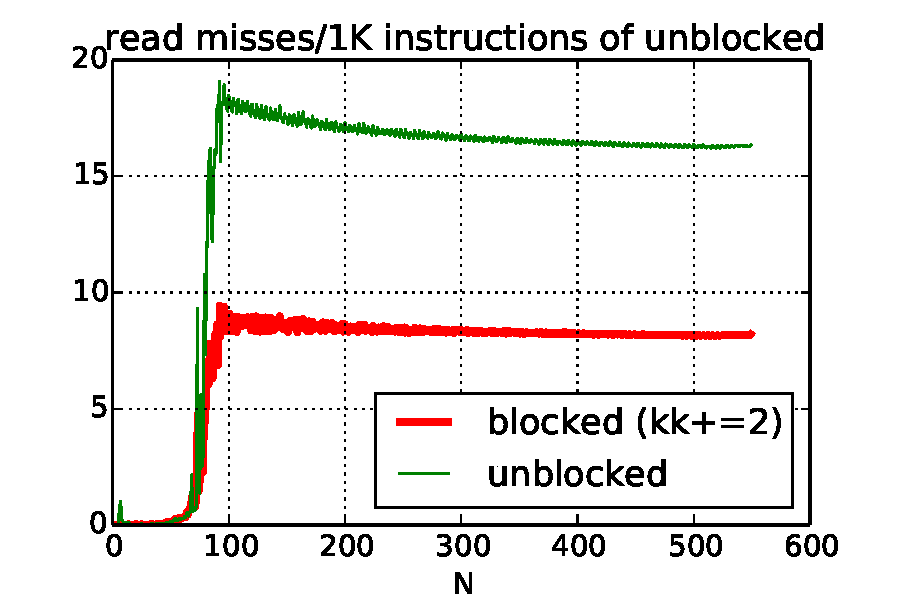
\includegraphics[width=0.8\textwidth]{../caching/k-kk-novec-block-read_miss_rate}
\end{frame}


\begin{frame}[fragile,label=cacheBlockExamplePartial]{simple blocking (2)}
\lstset{
    style=small,language=C,escapechar=@,
    moredelim=**[is][\btHL<2>]{~2}{~},
    moredelim=**[is][\btHL<3>]{~3}{~},
    moredelim=**[is][\btHL<4>]{~4}{~},
}
\begin{itemize}
\item same thing for $i$ in addition to $k$?
\end{itemize}
\begin{lstlisting}
for (int kk = 0; kk < N; kk += 2) {
  for (int ii = 0; ii < N; ii += 2) {
    for (int j = 0; j < N; ++j) {
      /* process a "block": */
      for (int k = kk; k < kk + 2; ++k)
        for (int i = 0; i < ii + 2; ++i)
            B[i*N+j] += A[i*N+k] * A[k*N+j];
    }
  }
}
\end{lstlisting}
\end{frame}

\begin{frame}[fragile,label=cacheBlockExamplePartialExpand]{simple blocking --- expanded}
\lstset{style=small,language=C,escapechar=@}
\begin{lstlisting}
for (int k = 0; k < N; k += 2) {
  for (int i = 0; i < N; i += 2) {
    /* load a block around Aik */
    for (int j = 0; j < N; ++j) {
      /* process a "block": */
      @\normalsize$B_{i+0,j}$@ += @\normalsize$A_{i+0,k+0}$@ * @\normalsize\myemph{$A_{k+0,j}$}@
      @\normalsize$B_{i+0,j}$@ += @\normalsize$A_{i+0,k+1}$@ * @\normalsize$A_{k+1,j}$@
      @\normalsize$B_{i+1,j}$@ += @\normalsize$A_{i+1,k+0}$@ * @\normalsize\myemph{$A_{k+0,j}$}@
      @\normalsize$B_{i+1,j}$@ += @\normalsize$A_{i+1,k+1}$@ * @\normalsize$A_{k+1,j}$@
    }
  }
}
\end{lstlisting}
\begin{itemize}
\item<2-> Now $A_{kj}$ reused in inner loop --- more calculations per load!
\end{itemize}
\end{frame}

